%----------------------------------------------------------------------------------------
%	CHAPTER - RESEARCH METHOD
%----------------------------------------------------------------------------------------

\chapter{Research Method}

\label{Research Method}

In this chapter, the research methodology of this thesis is described. The goal is to find the most suitable research method (philosophy, approach, and strategy) to answer the \gls{mrq}.


%----------------------------------------------------------------------------------------
%	SECTION 1
%----------------------------------------------------------------------------------------

\section{Introduction}

The main purpose is to derive a design for the visualisation and interaction with multidimensional data in virtual reality based on literature review, which then is tested and verified with the development of a prototype virtual reality application. In the following sub-chapters, the methodology is broken down in its individual parts. Due to the high relevancy for practitioners, out of the different research strategies defined by \cite{Hevner2010}, design science is applied.

%----------------------------------------------------------------------------------------
%	SECTION 2
%----------------------------------------------------------------------------------------

\section{Philosophy}

The first layer of the research methodology is the research philosophy, which shows how the researcher views the world and the knowledge that has to be developed as well as its nature.

\cite{Saunders2009} define four different research philosophies:
\begin{itemize}[noitemsep,nolistsep]
	\item Positivism \textit{(only observable phenomena will lead to the production of credible data)}
	\item Realism \textit{(do objects exist independently of our knowledge of their existence?)}
	\item Interpretivism \textit{(understanding differences between humans as social actors)}
	\item Pragmatism \textit{(do you have to adopt one position?)}
\end{itemize}

In addition, \cite{Saunders2009} also list three major ways of how to think about the different research philosophies:
\begin{itemize}[noitemsep,nolistsep]
	\item Epistemology \textit{(the view of the nature of reality or being)}
	\item Ontology \textit{(the view of what constitutes acceptable knowledge)}
	\item Axiology \textit{(the view of the role of values in research)}
\end{itemize}

A pragmatism research philosophy, as defined by \cite{Vaishnavi2008} and \cite{Saunders2009}, is assumed for this thesis since there is no decisive match for any of the other philosophies. The reason for this can be found upon evaluating the different views and philosophies. \newline
Since the design research will be tested and verified with the application of a prototype, this leads to the production of observable data which is an indication for the \textbf{positivism} philosophy. However, as the prototype will be used as part of a user testing, the results will be different based on the actors, leading also to an \textbf{interpretivism} philosophy. Due to this inconclusiveness, \cite{Saunders2009} see this as a confirmation for the application of the \textbf{pragmatism} philosophy, that unites the multi-philosophy approach into a dedicated one. \newline
By further looking at the views from \cite{Saunders2009}, the pragmatism philosophy can be further confirmed. From an \textbf{epistemology view}, both observable phenomena as well as subjective meanings are seen as acceptable knowledge and thus focus on the practical applied research \citep{Saunders2009}. This can be very well applied to this thesis as a combination of both observable data from the prototype as well as the subjective impression of the testers is considered important for the evaluation. In the \textbf{ontology view}, the researcher's view of the nature of reality is socially constructed, subjective and may change. In virtual reality, everything depends on how one perceives and interprets the visualizations; every individual has a different view of the (virtual) reality. This confirms the fact that \cite{Saunders2009} define a multi-view approach for the pragmatism philosophy. From the \textbf{axiology view}, the view of what role the values play, the researcher is part of what is being researched as he decides on his own how to interact with the \gls{ve}. This is subjective as it cannot be separated from the research and thus there will be not the one solution, but merely one out of many. 



%----------------------------------------------------------------------------------------
%	SECTION 3
%----------------------------------------------------------------------------------------

\section{Approach}

Based on \cite{Saunders2009}, a research approach can either be deductive (testing a theory), inductive (building a theory) or a combination of them. Table \ref{tbl:inductivedeductive} shows the major differences between deductive and inductive approach.
\begin{table}[h!]
	\begin{center}
		\begin{tabular}{ p{6.5cm} p{7.5cm} }
			\toprule
			\textbf{Deduction emphasises} & \textbf{Induction emphasises} \\
			\midrule
			Scientific principles & Less concern with the need to generalise \\
			Moving from theory to data & A close understanding of the research context  \\
			The need to explain causal relationships between variables & Gaining an understanding of the meanings humans attach to events \\
			The collection of quantitative data & The collection of qualitative data \\
			The application of controls to ensure validity of data & A realisation that the researcher is part of the research process \\
			The necessity to select samples of sufficient size in order to generalise conclusions & A more flexible structure to permit changes of research emphasis as the research progresses \\
			The operationalisation of concepts to ensure clarity of definition & \\
			A highly structured approach & \\
			Researcher independence of what is being researched & \\
			\bottomrule
		\end{tabular}
		\caption[Major differences between deductive and inductive approaches to research]{Major differences between deductive and inductive approaches to research (adopted from {\citealp[pg. 127]{Saunders2009}})}
		\label{tbl:inductivedeductive}
	\end{center}
\end{table} \newline
With literature review, knowledge about the current state of interaction possibilities with virtual reality as well as the visualization of data is collected and analysed. Based on the gained information and a close understanding of the research context, a theory can be formulated. With the help of a to be built prototype, this theory can be evaluated and tested by the researcher. This is a typical procedure of an inductive approach as described by \cite{Saunders2009}. \newline
The deductive approach starts at the other end as first the theory is built by searching to explain causal relationships between variables. The test of this theory requires the collection of quantitative data which is also part of this thesis as the testing and evaluation covers the actual functionality of the prototype as well. A theoretical approach for e.g. an interaction pattern is tested with the prototype for its practical application and functionality. \newline
\cite{Creswell2014} further defined a set of criteria for selecting a research approach based on the situation of current research. If only little research has been done yet and the topic first has to be explored and understood, then a qualitative (inductive) approach suits the best \citep{Creswell2014}. Although virtual reality in itself has been researched for more than a decade, it indeed is quite new to have full HD quality with gesture controllers available. This makes the thesis a good match for an inductive approach to create the design, the evaluation of it however is done in a quantitative (deductive) approach.


%----------------------------------------------------------------------------------------
%	SECTION 4
%----------------------------------------------------------------------------------------

\section{Strategy}

%-----------------------------------
%	SUBSECTION 1
%-----------------------------------

\subsection{Introduction}

\cite{Saunders2009} consider seven different research strategies:
\begin{itemize}[noitemsep,nolistsep]
	\item Experiment \textit{(study causal links)}
	\item Survey \textit{(answering who, what, where, how much and how many questions)}
	\item Case Study \textit{(empirical investigation within its real life context)}
	\item Action Research \textit{(explicit focus on research in action)}
	\item Grounded Theory \textit{(emphasis upon developing and building a theory)}
	\item Ethnography \textit{(describe and explain the social world the research subjects inhabit)}
	\item Archival Research \textit{(administrative records and documents as principle data source)}
\end{itemize}
In Information Systems, \cite{Hevner2010} suggest \textbf{design science} as another research strategy which inherently is a problem solving process. For this strategy, seven guidelines for design science research are derived which can be summarized in two main characteristics \citep{Hevner2010}: On the one hand the creation of an innovative, purposeful artefact for a specified problem domain, and on the other hand the thorough evaluation of the artefact and its high applicability in practice. Both of them are considered crucial for this thesis. \newline
The artefact is represented by the prototype of a \gls{vr} application that utilizes its input methods and interaction patterns compared to traditional non\gls{vr}approach. The relevance for practice and its applicability is given by feasible enhancements to solutions that are already used in practice.


%-----------------------------------
%	SUBSECTION 2
%-----------------------------------

\subsection{Design Research Cycle}

\label{DSRCycle}

\cite{Vaishnavi2008} and \cite{Hevner2010} define \gls{dsr} as a research paradigm in which questions that are relevant to human problems are answered with the creation of innovative artefacts. As an approach for conducting design science research, \cite{Vaishnavi2004} defined a design science research process model (\gls{dsr} Cycle). This cycle follows a step-wise approach and has been structured in the five phases that are as follows: \textit{Awareness of the Problem}, \textit{Suggestion}, \textit{Development}, \textit{Evaluation} and \textit{Conclusion} (Figure \ref{fig:dsrcycle}). In the following chapters, these five phases and their relation to this thesis are discussed.
\begin{figure}[h]
	\begin{center}
		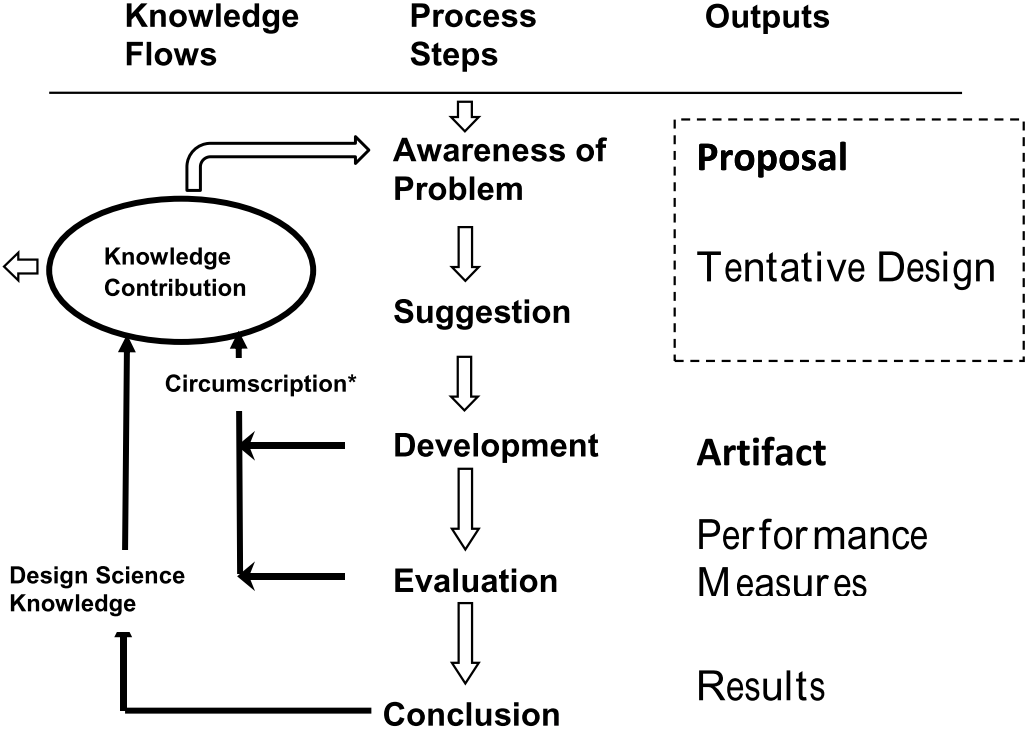
\includegraphics[width=11cm]{03_Figures/02_DSR_Cycle/DSR_Cycle.png}
		\caption[Design Science Research Process Model (\gls{dsr} Cycle)]{Design Science Research Process Model (\gls{dsr} Cycle) \citep{Vaishnavi2004}}
		\label{fig:dsrcycle}
	\end{center}
\end{figure}


%-----------------------------------
%	SUBSUBSECTION 1
%-----------------------------------

\subsubsection{Awareness}

\cite{Hevner2010} defined in the initial step of the \gls{dsr} Cycle the awareness of the problem, where
\begin{itemize}[noitemsep,nolistsep]
	\item the problem is identified.
	\item the problem is defined.
	\item the value of a solution is justified.
\end{itemize}
This is the foundation of all subsequent steps as the \textit{Suggestion}, \textit{Development} and \textit{Evaluation} phase all focus on the identified problem. \newline
In this thesis, the identification and definition of the problem is covered in Chapter \ref{ChapterIntroduction} (Introduction) whereas the justification of the value of a solution is established in the literature of Chapter \ref{ChapterLiteratureReview} in the form of research gaps.
The literature review shows that while there has been research done on the interaction patterns for \textit{Travel} and \textit{Selection}, the \textit{Motivation} is only covered on the surface. Furthermore, although guidelines for the interaction patterns are available, there are no practical suggestions/recommendations on how this could look like in practice or whether these guidelines really make sense once applied. The motivation for an improvement lies in the importance of \textit{Manipulation} patterns or uses in practice and recommendations on how matching interactions patterns have to be designed with the corresponding method in mind.


%-----------------------------------
%	SUBSUBSECTION 2
%-----------------------------------

\subsubsection{Suggestion}

\cite{Hevner2010} defined that in this phase, a preliminary suggestion for a solution is created, which is based on the knowledge gathered from the Literature Review in Chapter \ref{ChapterLiteratureReview}. \gls{srq} 1 and 2 will build the foundation for the selection of the right input method and interaction pattern whereas \gls{srq} 3 focuses on strategies for data visualisation and manipulation \newline
The general architecture of the prototype will be based on general knowledge from software engineering and the utilization of the \gls{sdk} and framework provided by Unity 3D.


%-----------------------------------
%	SUBSUBSECTION 3
%-----------------------------------

\subsubsection{Development}

In the development phase, the existing knowledge together with the defined problem definition is synthesized into an artefact that solves the mentioned problem \citep{Vaishnavi2008}. In this thesis, the artefact is the virtual reality prototype application.


%-----------------------------------
%	SUBSUBSECTION 4
%-----------------------------------

\subsubsection{Evaluation}

\label{EvaluationMethodology}

In order to demonstrate that with the proposed solution the problem can be solved, \cite{Hevner2010}  defined that the artefacts needs to be evaluated. Table \ref{tbl:designevaluationmethods} shows possible evaluation methods for designed artefacts that are based on \cite{Hevner2004}. \newline
For this research, the methods from \textit{Testing} and \textit{Descriptive} will be applied (also highlighted in Table \ref{tbl:designevaluationmethods}). The observational methods are not considered due to the limited time available for this research and the fact that the artefact will only be a prototype. The analytical and experimental methods do not fit since the focus of this research is rather a proof of concept than a full analysis which would also include sociological aspects (i.e. complexity or usability) which are not part of this research.\newline
The \textbf{testing} evaluation methods can be used to find weaknesses and identify defects in the system. Structural White Box Testing is performed during the development of the artefact whereas the Functional Black Box Testing will be performed afterwards for the integration (functional) acceptance. \newline
Since the focus of this research is to build a prototype solution for an existing problem, the \textbf{descriptive} evaluation methods help to prove the functionality and usefulness in the real-life context by validating it in scenarios. Due to the time restrictions, the scenario evaluation will be done subjectively as a long-term study with a greater amount of test persons is not deemed feasible.

\begin{table}[h]
	\begin{center}
		\begin{tabular}{ | m{4cm} | p{10cm} | } 
			\hline
			\multirow{2}{*}{1. Observational} &
			Case Study: Study artefact in depth in business environment \\
			\cline{2-2}
			& Field Study: Monitor use of artefact in multiple projects \\
			\hline
			\multirow{8}{*}{2. Analytical} &
			Static Analysis: Examine structure of artefact for static qualities (e.g., complexity) \\
			\cline{2-2}
			& Architecture Analysis: Study fit of artefact into technical IS architecture \\
			\cline{2-2}
			& Optimization: Demonstrate inherent optimal properties of artefact or provide optimality bounds on artefact behaviour \\
			\cline{2-2}
			& Dynamic Analysis: Study artefact in use for dynamic qualities (e.g., performance) \\
			\hline
			\multirow{3}{*}{3. Experimental} &
			Controlled Experiment: Study artefact in controlled environment for qualities (e.g., usability) \\
			\cline{2-2}
			& Simulation - Execute artefact with artificial data \\
			\hline
			\multirow{5}{*}{4. Testing} &
			\cellcolor{green!25}\textbf{Functional (Black Box) Testing:} Execute artefact interfaces to discover failures and identify defects \\
			\hhline{|~|-|}
			& \cellcolor{green!25}\textbf{Structural (White Box) Testing:} Perform coverage testing of some metric (e.g. execution paths) in the artefact implementation \\
			\hline
			\multirow{5}{*}{5. Descriptive} &
			\cellcolor{green!25}\textbf{Informed Argument:} Use information from the knowledge base (e.g. relevant research) to build a convincing argument for the artefact's utility \\
			\hhline{|~|-|}
			& \cellcolor{green!25}\textbf{Scenarios:} Construct detailed scenarios around the artefact to demonstrate its utility \\
			\hline
		\end{tabular}
		\caption[Design Evaluation Methods]{Design Evaluation Methods \citep[based on][]{Hevner2004}}
		\label{tbl:designevaluationmethods}
	\end{center}
\end{table}


%-----------------------------------
%	SUBSUBSECTION 5
%-----------------------------------

\subsubsection{Conclusion}

In the conclusion, the final phase of the \gls{dsr} Cycle, a consolidated overview of the work, the gained knowledge and the results are presented. In addition, suggestions for future research will be given.


%----------------------------------------------------------------------------------------
%	SECTION 5
%----------------------------------------------------------------------------------------

\section{Timeline}

As part of the master thesis research proposal, the literature review is conducted alongside its analysis. The development and evaluation of the prototype as part of the design science research will be done in the implementation phase of the master thesis.\newline
\cite{Saunders2009} distinguish between the \textit{cross-sectional} and the \textit{longitudinal} perspective. While the cross-sectional perspective covers a "snapshot" taken at a particular time, the longitudinal perspective covers a longer period of time \citep{Saunders2009}. Due to the limited available time for this research, the \textbf{cross-sectional} perspective is chosen.


%----------------------------------------------------------------------------------------
%	SECTION 6
%----------------------------------------------------------------------------------------

\section{Data collection}

In research, data collections is categorized as either quantitative (numeric, numbers) or qualitative (non-numeric, words), it however can also be mixed \citep{Saunders2009}. While quantitative data primarily includes questionnaires, graphs or statistics, qualitative data goes from interviews to data analysis and also include other data such as pictures and video clips \citep{Saunders2009}. The different techniques and procedures are further categorized into two main research choices: mono method and multiple methods, where the latter is further broken down into multi-method and mixed-method \citep{Saunders2009}. By implementing a prototype to evaluate the research design, the results will solely consist of quantitative data collected from the hands-on application: the implementation either works or it does not. Based on this, the \textbf{mono method} research is deemed the most applicable one.



%----------------------------------------------------------------------------------------
%	SECTION 7
%----------------------------------------------------------------------------------------

% \section{Data analysis}


%----------------------------------------------------------------------------------------
%	SECTION 8
%----------------------------------------------------------------------------------------

\section{Conclusion}

Since an artefact with high relevance for the practice is developed, design research has been found to be the best strategy for this research. The literature review covers the awareness of the problem and gives an indication for a to be suggested design. In the subsequent chapters, this will be further fostered into a clear suggestion for the prototype (Chapter \ref{ChapterSuggestion}). This prototype then is developed (Chapter \ref{ChapterDevelopment}) and evaluated with user testing (Chapter \ref{ChapterEvaluation}). These results then are further analysed and will form the conclusion in Chapter \ref{ChapterConclusion}.
